%% ===========================================
%% Nation-wise Failure Distribution - Top Conf Quality
%% Version 3 (Final) - Camera-Ready
%% ===========================================

\documentclass[tikz,border=3pt]{standalone}
\usepackage{tikz}
\usepackage{pgfplots}
\pgfplotsset{compat=1.18}
\usetikzlibrary{calc, positioning, arrows.meta, decorations.pathreplacing}

% Colorblind-safe palette (Okabe-Ito based)
\definecolor{c_nonlatin}{RGB}{230,159,0}    % orange
\definecolor{c_ocr}{RGB}{86,180,233}        % sky blue
\definecolor{c_math}{RGB}{204,121,167}      % reddish purple
\definecolor{c_reason}{RGB}{0,114,178}      % strong blue
\definecolor{c_other}{RGB}{180,180,180}     % neutral gray

\begin{document}

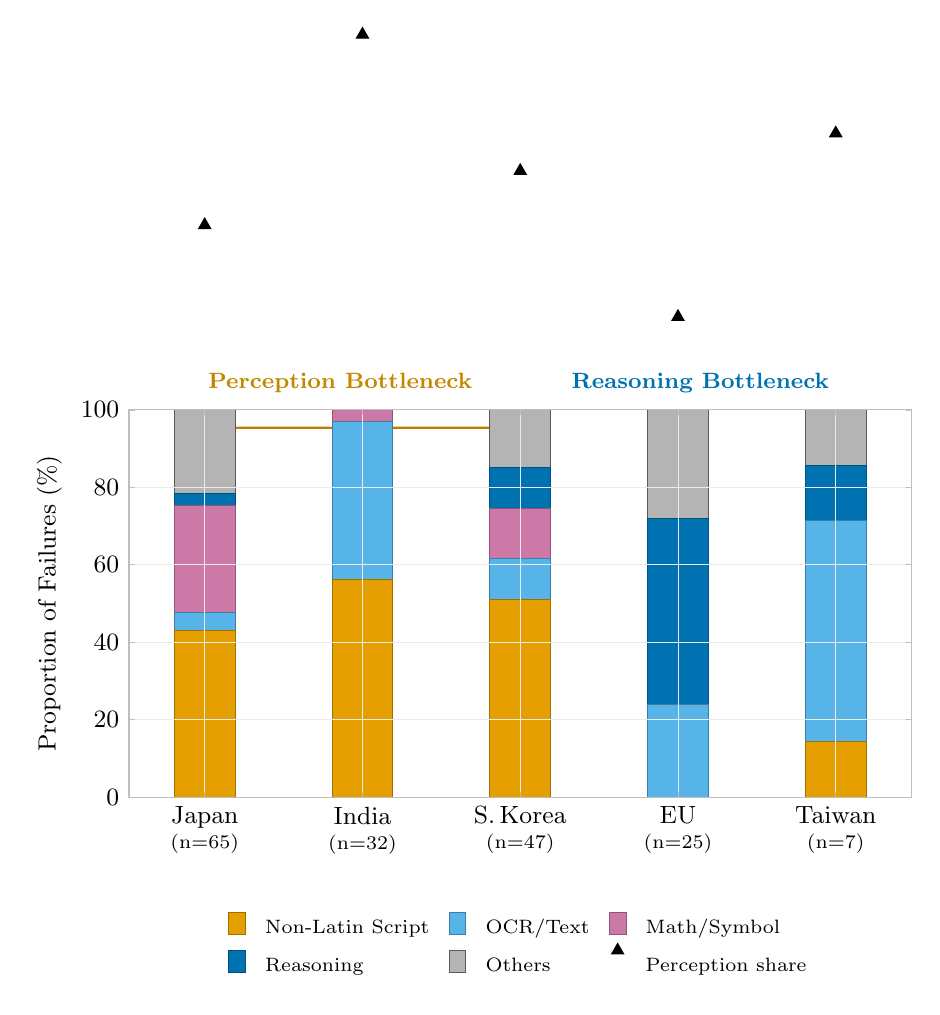
\begin{tikzpicture}
\begin{axis}[
    ybar stacked,
    bar width=22pt,
    width=0.95\columnwidth,  % paper-safe sizing
    height=6.5cm,
    ylabel={Proportion of Failures (\%)},
    ymin=0,
    ymax=100,
    ytick={0,20,40,60,80,100},
    xtick=data,
    symbolic x coords={Japan, India, S.Korea, EU, Taiwan},
    xticklabels={
        {Japan\\[-2pt]{\scriptsize(n=65)}},
        {India\\[-2pt]{\scriptsize(n=32)}},
        {S.\,Korea\\[-2pt]{\scriptsize(n=47)}},
        {EU\\[-2pt]{\scriptsize(n=25)}},
        {Taiwan\\[-2pt]{\scriptsize(n=7)}}
    },
    xticklabel style={align=center, font=\small},
    y tick label style={font=\small},
    ylabel style={font=\small},
    legend style={
        at={(0.5,-0.28)},
        anchor=north,
        legend columns=3,
        font=\scriptsize,
        column sep=5pt,
        draw=none,
    },
    legend cell align={left},
    enlarge x limits=0.12,
    clip=false,
    axis on top,
    grid=major,
    major grid style={gray!15, line width=0.3pt},
    axis line style={gray!50},
    tick style={gray!50},
    major tick length=2pt,
]

% Non-Latin Script (orange)
\addplot+[
    ybar stacked,
    fill=c_nonlatin,
    draw=c_nonlatin!70!black,
    line width=0.3pt,
] coordinates {
    (Japan, 43.1)
    (India, 56.3)
    (S.Korea, 51.1)
    (EU, 0)
    (Taiwan, 14.3)
};

% OCR/Text Recognition (sky blue)
\addplot+[
    ybar stacked,
    fill=c_ocr,
    draw=c_ocr!70!black,
    line width=0.3pt,
] coordinates {
    (Japan, 4.6)
    (India, 40.6)
    (S.Korea, 10.6)
    (EU, 24.0)
    (Taiwan, 57.1)
};

% Math/Symbol (purple)
\addplot+[
    ybar stacked,
    fill=c_math,
    draw=c_math!70!black,
    line width=0.3pt,
] coordinates {
    (Japan, 27.7)
    (India, 3.1)
    (S.Korea, 12.8)
    (EU, 0)
    (Taiwan, 0)
};

% Pure Reasoning (strong blue)
\addplot+[
    ybar stacked,
    fill=c_reason,
    draw=c_reason!70!black,
    line width=0.3pt,
] coordinates {
    (Japan, 3.1)
    (India, 0)
    (S.Korea, 10.6)
    (EU, 48.0)
    (Taiwan, 14.3)
};

% Others (gray)
\addplot+[
    ybar stacked,
    fill=c_other,
    draw=c_other!50!black,
    line width=0.3pt,
] coordinates {
    (Japan, 21.5)
    (India, 0)
    (S.Korea, 14.9)
    (EU, 28.0)
    (Taiwan, 14.3)
};

% Perception share markers (Non-Latin + OCR) - integrated into legend
\addplot+[
    only marks,
    mark=triangle*,
    mark size=2.5pt,
    mark options={fill=black, draw=black},
] coordinates {
    (Japan, 47.7)
    (India, 96.9)
    (S.Korea, 61.7)
    (EU, 24.0)
    (Taiwan, 71.4)
};

\legend{
    Non-Latin Script,
    OCR/Text,
    Math/Symbol,
    Reasoning,
    Others,
    Perception share
}

% ===== Key annotations (dark text on light fills, white on dark) =====

% Japan: Non-Latin 43% (dark text on orange)
\node[font=\scriptsize\bfseries, text=black] at (axis cs:Japan, 21.5) {43\%};

% India: Non-Latin 56% + OCR 41%
\node[font=\scriptsize\bfseries, text=black] at (axis cs:India, 28) {56\%};
\node[font=\scriptsize\bfseries, text=black] at (axis cs:India, 77) {41\%};

% S.Korea: Non-Latin 51%
\node[font=\scriptsize\bfseries, text=black] at (axis cs:S.Korea, 25.5) {51\%};

% EU: Reasoning 48% (white text on dark blue)
\node[font=\scriptsize\bfseries, text=white] at (axis cs:EU, 48) {48\%};

% ===== Bottleneck annotations (using axis description cs for stability) =====

% Perception Bottleneck brace (Japan to S.Korea)
\draw[decorate, decoration={brace, amplitude=5pt, raise=4pt, mirror}, 
      thick, c_nonlatin!80!black]
    (axis cs:Japan, 100) -- (axis cs:S.Korea, 100);

\node[font=\footnotesize\bfseries, c_nonlatin!85!black, align=center,
      anchor=south] 
    at (axis description cs:0.27, 1.02) 
    {\textsc{Perception Bottleneck}};

% Reasoning Bottleneck label for EU (using arrow)
\draw[-{Stealth[length=4pt]}, line width=0.7pt, c_reason]
    (axis cs:EU, 80) -- (axis cs:EU, 54);
\node[font=\footnotesize\bfseries, c_reason, anchor=south] 
    at (axis description cs:0.73, 1.02) 
    {\textsc{Reasoning Bottleneck}};

\end{axis}
\end{tikzpicture}

\end{document}
